\begin{sectionbox}
    \subsection{Moleküle - Bindungstypen}
    Bindungen entstehen nur, wenn die Energie des Moleküls geringer als die Energie der Einzelatome sein wird. \\
    \fboxsep0pt\colorbox{lightgreen}{\parbox{\columnwidth}{
            \begin{tabular*}{\columnwidth}{@{\extracolsep\fill}lll@{}}
                \ctrule
                Bindung & Eigenschaften & Energie \\\cmrule
                Ionisch & Elektronaustausch, stark, starr & $\SI{3.4}{\electronvolt}$ \\
                Kovalent & Gemeinsame Elektronen & \\
                Metallisch & "`Elektronensee"' &  \\
                Dipol & Coulombkräfte von Partialladungen  & \\
                \ctrule
            \end{tabular*}
        }}


    \subsubsection{Ionische Bindung }
    \underline{Voraussetzung}: unterschiedliche Atome, leicht zu ionisieren, Energieabgabe bei Bindung \\

    \begin{cookbox}{Ionisierung}
        \item Anion und Kation ziehen sich an bis auf einen Abstand der Ionenmittelpunkte: $r_0=(r_{\text{Y}^-}+r_{\text{X}^+})$
        \item Dabei wird die Energie frei: $E_{\ir el}= \int\limits_\infty^{r_0} \frac{-e^2}{4\pi\epsilon_0r^2 }\diff r= \frac{e^2}{4\pi\epsilon_0r_0}$
        %    	\item Bindungsenergie beträgt $\frac{\SI{3,4}{\electronvolt}}{\text{Ionenpaar}}$ oder $328\frac{\text{kJ}}{\text{Mol}}$
        \item Coulombanziehung nicht gerichtet $\rightarrow$ positive und negative Ionen lagern so dicht aneinander wie möglich $\rightarrow$ Ionenkristall (nicht verformbar)
        \item Elektronen sind an den Ionen lokalisiert $\rightarrow$ keine freien Elektronen vorhanden $\ra $ Isolator
        \item Differenz der Elektronegativität meist $\Delta E>1.7$
        \item Gesamtbilanz der der Ionischen Bindung\\
        X + $E_X \rightarrow \text X^+ + \e^-$\\
        Y + $\e^- \rightarrow \text Y^- + E_Y$\\
        $\text X^+ + \text Y^- \rightarrow \text{XY} + E_{\ir el}$\\
        $E_{\ir ges} = -E_X + E_Y + E_{\ir el}$\\
    \end{cookbox}


    \subsubsection{Kovalente Bindung}
    Spinabsättigung der äußeren Elektronenschale durch \textbf{gemeinsame Elektronen}

    \begin{itemize}
        \item Valenz-Elektronen zwischen den Atomen lokalisiert
        \item keine Kugelsymmetrische Ladungsverteilung mehr im Atom
        \item Die Anzahl der Elektronen mit umgepaartem Spin zeigt an wie vielfache kovalente Bindungen eingegangen werden können
        \item treten bei und zwischen Elementen der IV. bis VII. Hauptgruppe (+H) auf
        \item gerichtete Bindungen $\rightarrow$ mögliche Kristallstrukturen werden eingeschränkt
        \item Differenz der Elektronegativität meist $\Delta E<1.7$
        \item kovalente gebundene Kristalle sind üblicherweise schlechte Leiter
    \end{itemize}


    \subsubsection{Metallische Bindung}
    Sonderfall der kovalenten Bindung, bei der die Valenz-Elektronen nicht lokalisiert sind.
    \begin{itemize}
        \item Vorwiegend Elemente mit nur wenigen Außenelektronen
        \item freie Elektronen $\ra $ hohe elektrische Leitfähigkeit, hohe Wärmeleitfähigkeit
        \item Bindung nicht gerichtet $\rightarrow$ hohe Packungsdichte
        \item Bindungen mit gleich- und ungleichartigen Metallen eingegangen werden
        \item Metallische Bindung ist schwächer als die ionische oder kovalente Bindung
        \item Bindungsstärke hängt von der Zahl der Leitungselektronen ab
    \end{itemize}

    \subsubsection{Dipolbindung}
    \begin{itemize}
        \item zwischen Molekülen mit permanentem Dipolmoment $\rightarrow$ Moleküle mit positiver und negativer Ladung
        \item Dipole ordnen sich im Dipolfeld der Nachbaratome so an, dass möglichst geringe Abstand und durch die Coulombkräfte gebunden werden
    \end{itemize}

    \subsubsection{Van-der-Waals-Bindung:}
    \begin{itemize}
        \item Atome/Moleküle haben kein permanentes Dipolmoment
        \item Bindung zwischen Dipolen durch statistische Fluktuationen der Ladungsschwerpunkte.
        \item Sehr schwache Bindung
    \end{itemize}
    \subsubsection{Wasserstoffbrückenbindung}
    \underline{Vorraussetzung:} Äußere Schale $>$ vier Elektronen, zwischen 2 Atomen.
    \begin{itemize}
        \item Bindungen über Wasserstoffbrücken der Form A-H-A
        \item Das H-Atom geht eine kovalente Bindung mit Atom der Sorte A ein und gibt sein Elektron ab. Das Proton bleibt fest an Reaktionspartner gebunden und bindet nun zusätzlich das andere negative Atom
        \item Bindungsenergie ist gering $(\SI{0,1}{\electronvolt})$
    \end{itemize}

    \subsubsection{Kristallstrukturen}
    TODO 3.4

\end{sectionbox}



\begin{sectionbox}
    \subsection{Das Periodensystem}
    \fboxsep0pt\colorbox{lightgreen}{\parbox{\columnwidth}{

            \begin{tabularx}{\linewidth}{@{}>{\bfseries}l@{\hspace{.5em}}X@{}}
                \ctrule
                Hauptquantenzahl    &
                $n = 1, 2, \ldots (= $ K, L, \ldots - Schale$)$                                                                                       \\
                                    & bestimmt die Energie, $n > l$                                                                                   \\
                Bahndrehimpulsqz.   &
                $l = 0, \ldots, n-1$ (= s,p,d,f - Zuständen)                                                                                          \\
                                    & bestimmt die Form der Wellenfkt.                                                                                \\
                Magnet. Quantenzahl &
                $m \in [-l, l]$                                                                                                                       \\
                                    & $|[-l, l]|$ bestimmt Anzahl der Orbitale für geg. $l$: $l=1\Rightarrow |[-1,1]|=3 \Rightarrow 3$ (p) - Orbitale \\
                Spinquantenzahl     &
                $s = \pm \frac{1}{2} \quad$ Eigendrehimpuls des Elektrons                                                                             \\
                \ctrule
            \end{tabularx}
        }}
    Zu jedem Wert n gehören $n^2$ Zustände selber Energie durch Variation von $l$ und $m$. Außerdem ist jeweils ein Spin $s = \pm \frac 1 2$ möglich.\\
    \textbf{Entartungsgrad:} Zustände selber Energie: $2 n^2$ \\
    \textbf{Grundzustand:} $n=1, m=0, l=0$ \\
    \textbf{Orbital:} Bereich eines Atoms, welcher genau 2 Elektronen unterschiedlichen Spins halten kann
    \textbf{Energie-Eigenwerte des Wasserstoffatoms:}\begin{equation*}
        E_n=-\frac{\hbar^2}{2m_0}\left(\frac{1}{na_0}\right)^2=-\frac{m_0e^4}{2(4\pi\epsilon_0 \hbar)^2}\frac{1}{n^2}
    \end{equation*}
\end{sectionbox}


%=======================================================================
\begin{sectionbox}
    \subsection{Atome - Hundsche Regeln}
    Legen fest, nach welchem Schema Orbitale derselben Energie (gleichem $n$) eines Atoms mit Elektronen besetzt wird.
    \begin{enumerate}
        \item Orbitale derselben Energie werden zunächst mit demselbem Spin ausgerichtet, bis jedes der Orbitale halb gefüllt ist. Erst danach wird der andere Platz durch ein Elektron mit anderem Spin ausgefüllt
        \item Gesamtdrehinmpuls $\abs{L} = \abs{\sum m_i} = \max$
        \item Falls die Schale weniger als halbvoll ist:
              \begin{itemize}
                  \item Bahndrehimpuls und Spin antiparallel
                  \item Gesamtdrehimpuls $J$: $\abs{J} = \abs{\abs{L} - \abs{S}}$
              \end{itemize}
              Falls die Schale mehr als halbvoll ist:
              \begin{itemize}
                  \item Bahndrehimpuls und Spin parallel
                  \item Gesamtdrehimpuls $J$: $\abs{J} = \abs{\abs{L} + \abs{S}}$
              \end{itemize}
    \end{enumerate}
    Merke: Volle Schalen liefern keinen Beitrag zu $S$, $L$ und $J$
    \paragraph{Pauli-Prinzip:}
    Alle Elektronen unterscheiden sich in mindestens einer Quantenzahl
    \begin{center}
        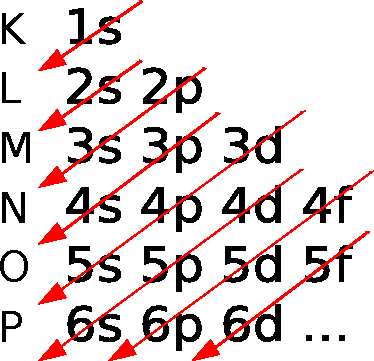
\includegraphics[width = 2cm]{./img/klechkovski.pdf}
    \end{center}
    { \fboxsep0.2em
        \begin{tabular}{c|ccc}
            ${}_{\color{red}\displaystyle \boldsymbol{n}}\!{\LARGE \diagdown}\!{}^{\color{blue}\displaystyle \boldsymbol{l}}$ & \color{blue}$0 =\textbf{s}$ & \color{blue}$1 = \textbf{p}$                                                      & \color{blue}$2 = \textbf{d}$                                                                                                            \\ \mrule
                                                                                                                              & $m = 0$                     & $m=-1,0,1$                                                                        & $m=-2,-1,0,1,2$                                                                                                                         \\
            \color{red}1:K                                                                                                    & \fbox{$\uparrow\downarrow$} &                                                                                                                                                                                                                             \\[0.2em]
            \color{red}2:L                                                                                                    & \fbox{$\uparrow\downarrow$} & \fbox{$\uparrow\downarrow$}\fbox{$\uparrow\downarrow$}\fbox{$\uparrow\downarrow$}                                                                                                                                           \\[0.2em]
            \color{red}3:M                                                                                                    & \fbox{$\uparrow\downarrow$} & \fbox{$\uparrow\downarrow$}\fbox{$\uparrow\downarrow$}\fbox{$\uparrow\downarrow$} & \fbox{$\uparrow\downarrow$}\fbox{$\uparrow\downarrow$}\fbox{$\uparrow\downarrow$}\fbox{$\uparrow\downarrow$}\fbox{$\uparrow\downarrow$} \\
        \end{tabular} }
\end{sectionbox}

TODO: Gitterstrukturen, Bindungen genauer